\documentclass[letterpaper]{article}
\usepackage{amsmath, geometry, graphicx, tikz}
\usetikzlibrary{arrows.meta}
\bibliographystyle{plain}

\title{Aging and genomic imprinting in the human brain}
\author{First Author 1, First Author 2, Middle Author,..., Middle Author, Andrew
Chess}

\begin{document}
\maketitle

\begin{abstract}
Lorem ipsum...
\end{abstract}

\section{Introduction}

Variation of expression level across genes, lifetime, cells, tissue types, as
well as individuals in the human population is clearly a major determinant of
phenotype REF.  A distinct, though related, question is the role of the
\emph{ratio} between maternal (or paternal) transcripts and those from both
alleles of a given gene.  Besides the random thermal fluctuations, which occur
in all genes, some genes display systematic \emph{parental bias} in allelic
expression.  The extreme form of this bias is known as monoallelic expression,
which may be non-random if expression is biased towards only one parent or
random otherwise \cite{Chess2012}.

Genomic imprinting is the classic, non-random, case of monoallelic expression,
which is mediated by epigenetic mechanisms that either concern single genes or
entire imprinted gene clusters.  Having emerged late in evolution, imprinting
of several genes have been implicated in biological functions of mainly
neurological, psychological, behavioral and social type.  Mutations disrupting
the expression of certain imprinted genes are deeply penetrant causes of rare
syndromes displaying psychological, cognitive, and social dysfunction.  But it
remains to be established to what extent more subtle perturbations of parental
bias might contribute to common, highly polygenic psychiatric disorders such
as schizophrenia or autism.

Also of interest is how and why parental bias for a given imprinted gene
might vary between individuals.  Age is a prime candidate for regulator
given that several imprinted genes have been found to be functionally associated to either
perinatal stage (e.g.~suckling) or young adulthood (e.g.~maternal care).
Gender and ancestry are obvious further candidates.

A modern approach to study the variation of parental bias is to differentiate
maternal and paternal transcripts based on those single nucleotide
polymorphisms (SNPs) that contribute to the heterozygosity of a given
individual and gene.  Coupled with high throughput techniques such as RNA-seq
this approach permits the quantification of both genome-wide and
among-individual variation.  Several research groups
\cite{Gregg2010a,Perez2015,DeVeale2012} combined this approach with F1 hybrids
of crossed mouse strains and found, for instance, that \(\approx 1\%\) of all
genes are imprinted, although some \cite{Perez2015} of the same researchers
previously estimated \(> 5\%\), leaving this question controversial.
Another finding is the differential effect of age, but not gender, on parental
bias: shifting from neonatal age to young adulthood down-regulated bias in
ca.~\(20\%\) of detected imprinted genes, up-regulated in \(6\%\) and had no
effect on the remaining nearly \(75\%\).

While such designed mouse experiments afford high statistical power their
relevance is at best unclear to human neuropsychological function, ageing and
ancestry.  The present work directly addresses these points by utilizing
post-mortem tissue samples from the dorsolateral prefrontal cortex (DLFPC)
from nearly 600 individuals of different age, psychiatric condition, and
ancestry, and by performing the RNA-seq based quantification of parental bias.

\section{Methods}

\subsection{Data}

\(m\) individuals/samples, set \(\mathcal{G}\) of \(n\) genes

\begin{table}
\begin{center}
\begin{tabular}{r|l}
predictor & parameter(s)\\
\hline
Age & Age\\
Institution & [MSSM], Penn, Pitt\\
Gender & [Female], Male\\
PMI & PMI\\
Dx & [AFF], Control, SCZ\\
RIN & RIN\\
RIN2 & RIN2\\
RNA\_batch & [0], A, B, C, D, E, F, G, H\\
Ancestry.1 & Ancestry.1\\
\vdots & \vdots \\
Ancestry.5 & Ancestry.5\\
\end{tabular}
\caption{}
\label{tab:predictors}
\end{center}
\end{table}

\subsection{Read count ratio: an estimate of parental bias}

\(\mathbf{S} = [S_{ig}]_{ig};\; i=1,...,m; \; g\in\mathcal{G}\)

\begin{equation}
S_{ig} = \frac{H_{ig}}{T_{ig}}= \frac{\sum_s H_s}{\sum_sT_s}
\end{equation}

\subsection{Regression models to explain population-wide variation}

Regression analysis involved a subset \(\mathcal{G}_1\subset\mathcal{G}\) of
\(n_1\) genes.

The basic model, unlm.S, is
\begin{eqnarray}
\mathbf{S} &=& \mathbf{X} \boldsymbol{\beta} + \boldsymbol{\varepsilon},
\label{eq:unlm.S-matrix-form} \\
\varepsilon_{ig} &\overset{\mathrm{iid}}{\sim}& \mathrm{Norm}(0, \sigma^2_g)
\end{eqnarray}
where the response \(\mathbf{S}\) is an \(m\times n_1\) matrix of read count ratios,
\(\mathrm{X}\) is an \(m\times p\) design matrix, \(\boldsymbol{\beta}\) is a \(p\times n_1\) matrix of regression
coefficients, the random error \(\boldsymbol{\varepsilon}\) has the same
dimension as \(\mathbf{S}\), and gene \(g\in \mathcal{G}_1\).  Eq.~\ref{eq:unlm.S-matrix-form} may be given as
\begin{equation}
S_g = \mathbf{X} \beta_g + \varepsilon_g,
\label{eq:unlm.S-vector-form}
\end{equation}
where the vectors \(S_g, \beta_g, \varepsilon_g\)
are single columns taken from their respective matrix counterparts.

unlm.S was extended in several ways, yielding
\begin{enumerate}
\item four normal linear models unlm.S, unlm.R, wnlm.S, wnlm.S
\item two logistic models logi.S and logi2.S.
\end{enumerate}

The general form of the four normal linar models
(cf.~\ref{eq:unlm.S-vector-form}) is
\begin{equation}
W_g^{1/2} \tau(S_g) = W_g^{1/2} X \beta_g + \varepsilon_g.
\label{eq:nlm-general}
\end{equation}
The extension here consists of \(W_g\), an \(m\times m\) diagonal matrix of
weights \(w_{ig}\) on the \(i\)-th diagonal position, and \(\tau\), a
transformation on read counts.  These quantities specify the four normal
linear models as laid out in Table~\ref{tab:nlm}.

\begin{table}
\begin{center}
\begin{tabular}{c|cc}
model & transformation \(\tau\) & weights \(w_{ig}\) \\
\hline
unlm.S & none & 1 \\
unlm.R & rank transf. & 1 \\
wnlm.S & none & \(T_{ig}\) \\
wnlm.R & rank transf. & \(T_{ig}\) \\
\end{tabular}
\end{center}
\caption{Specificiation of four normal linear models based on read count
transformation \(\tau\) and weights \(w_{ig}\).}
\label{tab:nlm}
\end{table}

The logistic models, logi.S or logi2.S, share the general form
\begin{eqnarray}
S_g &=& \mu_g + c\, \varepsilon_g
\label{eq:logi-general}
\\
\mu_g &=& h(X \beta_g) \\
\varepsilon_{ig} + \mu_g &\overset{\mathrm{iid}}{\sim}& \mathrm{Binom}(\mu_g, T_{ig}).
\label{eq:binom-error}
\end{eqnarray}
The link function \(h\) is \(h(u) = e^u / (1 + e^u)\) for logi.S and \(h(u) =
e^u / (2 + 2e^u)] + 1/2\) for logi2.S, and the scaling constant \(c=\) 1
 and \(1/2\), respectively.  Thus, the response \(S_g\) under logi2.S is scaled and shifted relative to
that under logi.S such that (with probabilty one) \(1/2\le S_{ig}\le 1\) under the former and
\(1/2\le S_{ig}\le 1\) under the latter.

Each of the six models has \(p\times n_1\) regression parameters corresponding to the
dimension of \(\boldsymbol{\beta}\).  This allows different behavior for
different genes since \(\beta_1\neq ...\neq\beta_{n_1}\) in general.
Therefore, the estimated regression coefficients are reported as \(\hat{\beta}_g =
(\hat{\beta}_{1g},...,\hat{\beta}_{jg},...,\hat{\beta}_{pg})\) for each gene \(g\), often
replacing index \(j\) with the name of the parameter such as \emph{Age} or
\emph{InstitutionPitt}.

A second set of six models was also
fitted, for which \(\boldsymbol{\beta}\) was constrained such that \(\beta_1 =
... = \beta_{n_1}\).  This was achieved by aggregating over genes
\(g\in\mathcal{G}_1\) the higher read count \(H'_i = \sum_g H_{ig}\), the
total read count \(T'_i = \sum_g T_{ig}\), redefining the read count ratio
as \(S'_i = H'_i / T'_i\), and replacing \(S_g\) by \(S'=(S'_1,...,S'_m)\) in
Eq.~\ref{eq:unlm.S-vector-form},~\ref{eq:nlm-general},~\ref{eq:logi-general}, and \(T_{ig}\) by \(T'_i\) in
Table~\ref{tab:nlm} and Eq.~\ref{eq:binom-error}.  Note that such aggregation
simplifies the matrix variables in Eq.~\ref{eq:unlm.S-matrix-form} to the
corresponding vector variables in Eq.~\ref{eq:unlm.S-vector-form}.  Because \(S'_i\) is a
weighted average of \(\{S_{ig}\}_i\), results under these models are reported
as \(\hat{\beta}_\mathrm{WA} =
(\hat{\beta}_{1\mathrm{WA}},...,\hat{\beta}_{j\mathrm{WA}},...,\hat{\beta}_{p\mathrm{WA}})\).  A
third set of models is a slight variation of this second set in that
aggregation was done on a smaller subset of 8 genes selected at the initial
stage of the study.  Under these models the results are reported using the
WA.8 subscript instead of WA.

These \(3\times 6\) models are all multiple regression ones with \(p<1\)
parameters.  Three corresponding sets of models with a single Age parameter
(\(p=1\)) were also fitted but the results were only used for graphical
comparison of model fits in terms of predictions
Fig.~\ref{fig:predicted-curves} but not for quantitative inference.

\section{Results}

\subsection{Genome-wide patterns}

Lorem ipsum

\begin{figure}
\begin{center}
\includegraphics[scale=0.6]{figures/2016-07-19-genome-wide-S/complex-plot-1.png}
\end{center}
\caption{}
\label{fig:ranking-genes}
\end{figure}

\begin{figure}
\begin{center}
\includegraphics[scale=0.6]{figures/2016-08-08-imprinted-gene-clusters/score-genomic-location-1.png}
\end{center}
\caption{}
\label{fig:clusters}
\end{figure}

\begin{figure}
\begin{center}
\includegraphics[scale=0.6]{figures/2016-08-01-ifats-filters/top-ranking-genes-1.pdf}
\caption{}
\label{fig:top-genes}
\end{center}
\end{figure}

\begin{figure}
\begin{center}
\includegraphics[scale=0.6]{figures/2016-06-26-trellis-display-of-data/S-age-smooth-1.png}
\caption{}
\label{fig:S-age-institution}
\end{center}
\end{figure}

\subsection{Modulation by age}

\begin{figure}
\begin{center}
\includegraphics[scale=0.6]{figures/2016-08-23-glm-sampling-distributions/GRB10-1.png}
\end{center}
\caption{}
\label{fig:predicted-curves}
\end{figure}

\begin{figure}
\begin{center}
\includegraphics[scale=0.6]{figures/2016-08-08-imprinted-gene-clusters/segplot-1.pdf}
\end{center}
\caption{}
\label{fig:age-effect}
\end{figure}

\begin{figure}
\begin{center}
\includegraphics[scale=0.6]{figures/2016-06-22-extending-anova/anova-effects-fw-rv-logi-S-1.pdf}
\end{center}
\caption{}
\label{fig:anova}
\end{figure}

\section{Discussion}

The main results of this work may be interpreted in terms of the scheme in
Fig.~\ref{fig:scheme}.  The scheme presents all \(n\) imprinted genes in a
tissue, such as the DLPFC, which is relevant to neural function.  Parental
bias is putatively regulated by age, gender, ancestry, and possibly other
biological factors.  The nature of regulation---simple up- or down-regulation,
no effect, or some more complex pattern---is captured in the functions
\(\psi_1,...,\psi_n\).  Function \(\phi\) maps jointly the \(n\) parental
biases to neuropsychology, and connects therefore the molecular phenotypic
level to the organismal one.

\begin{figure}[h]
\begin{center}
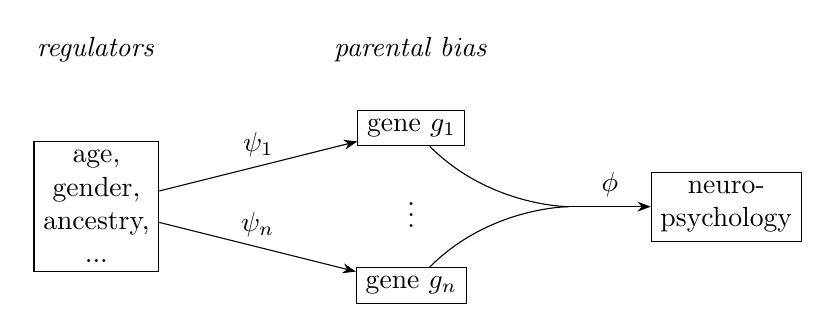
\begin{tikzpicture}[align=center]
\node at (-4,2) {\emph{regulators}};
\node[draw] (A) at (-4,0) {age,\\gender,\\ancestry,\\...};
\node at (0,2) {\emph{parental bias}};
\node[draw] (G1) at (0,1) {gene \(g_1\)};
\node at (0,0) {\vdots};
\node[draw] (Gn) at (0,-1) {gene \(g_n\)};
\coordinate (C) at (2,0);
\node[draw] (B) at (4,0) {neuro-\\psychology};
\draw[-Stealth] (A) -- node[anchor=south] {\(\psi_1\)} (G1);
\draw[-Stealth] (A) -- node[anchor=south] {\(\psi_n\)} (Gn);
\draw[-Stealth] (C) -- node[anchor=south] {\(\phi\)} (B);
\draw (G1) .. controls (1,0) and (2,0) .. (C);
\draw (Gn) .. controls (1,0) and (2,0) .. (C);
\end{tikzpicture}
\end{center}
\caption{}
\label{fig:scheme}
\end{figure}

Our genome-wide analysis suggests that \(<1\%\) of all genes are imprinted,
which implies \(n\approx 200\).  This provides evidence, in addition to
previous similarly conservative estimates of \(n\)
\cite{Perez2015,DeVeale2012}, against the controversial estimate of \(n\approx
1300\) \cite{Gregg2010a}.

More interestingly, we find that several regression coefficients differ
significantly from zero, which suggests that age, gender and ancestry do
indeed regulate parental bias in at least some imprinted genes in the human
DLPFC.  We infer that these three regulators exert gene-specific effects, up-
or down-regulating parental bias in a subset of imprinted genes while having
no (detectable) impact on the rest.  That these predictors differ in the
subset of genes they affect significantly hints at the potential complexity of
regulation.  A further layer of that complexity arises from possible
interactions among these predictors, which is in fact consistent with the
dependence of the age effect on gender in our conditional analysis.

The interpretation of the present results as the effect of (human) ancestry on
parental bias points to genetic regulatory mechanisms of imprinting that
modulate the known epigenetic mechanisms.  Given the late emergence of
imprinting in therian phylogeny and its role in neuropsychological and social
function, the genetics of parental bias may well be an increasingly important
target of natural selection.  Also, the ancestry effect is a remarkable
novelty of our work since previous studies, all using in-bread mouse strains,
failed to address this point.  As for age, a similar differential effect was
found in the mouse cerebellum to the effect we observe here. Gender, however,
had no significant effect in the same mouse study.

The above interpretation certainly depends on our statistical inference, which
in turn is based on the present data and regression models, both of which have
serious limitations.  Some of these---related to differing sequencing and
genotyping protocols---might be alleviated by improved across-institute
standardization.  But others, such as the confounding of age by certain
technical variables (e.g.~institution), are hopelessly entangled with the
observational nature of post mortem human studies, which precludes orthogonal,
that is clearly interpretable, decomposition of the variation in the observed
measure of parental bias (the response) into various technical and biological
components and limits statistical power.  Even if the data fulfilled
orthogonality, the present regression models would still remain too rigid to
account for the relative overdispersion of RNA-seq read counts, the
uncertainty surrounding haplotype, and that genes are neither completely
independent nor completely identical in their parental bias.  In future work
these ought to be tackled either with recently developed hierarchical models
built on normal linear model \cite{Perez2015,Law2014} or, if regulators indeed
strongly interact as the present work indicates, by the adoption of Bayesian
networks.

The molecular mechanism mediating the age effect.  TODO: clusters and regression
coefficients for gender and ancestry

Even if the regulatory effect of age, gender, ancestry, etc, on parental bias
is more firmly established by methodological improvements and more data, it
still remains to be determined whether (and how) the corresponding changes in
expression phenotype affect neural and psychological properties and might be
causal to some common psychiatric disorders.  This work may be considered an
initial step towards that aim as the estimated regression coefficients,
associated with SCZ or AFF, provide statistically weak hints at that
causality.

A more general question is how function \(\phi\) in Fig.~\ref{fig:scheme}
integrates parental bias across genes and maps that signal to organismal
phenotype.  That mapping occurs through the intermediate domain of cellular
metabolism.  Therefore, extending the present ``multi-omic'' data collection
with a metabolic layer appears promising, especially because rather specific
metabolism characterizes several imprinted genes \cite{Tucci2016,Peters2014}.
Adopting single-cell RNA-seq in the present framework would be another
interesting extension that could possibly elucidate the role of random
monoallelic expression.

In fact, the question regarding the map \(\phi\) is even more general, since
it is plausible that parental bias acts jointly with overall expression level
(this is not indicated in Fig.~\ref{fig:scheme}).  If so, the resolution of
the prevailing system biology is to be refined from mere genes to separate
maternal and paternal copies.  On the other hand, the present finding that
parental bias substantially varies across individuals even withing the same
tissue calls for a conceptual shift from the current practice of regarding
genes unconditionally as either imprinted or not to considering instead the
conditional distribution of their parental bias within the population given
regulators such as age, gender, and ancestry.

\bibliography{monoall-ms}

\section{Supplementary Material}

% Supplementary figures

\setcounter{figure}{0}
\makeatletter 
\renewcommand{\thefigure}{S\@arabic\c@figure}
\makeatother

\begin{figure}
\begin{center}
\includegraphics[scale=0.6]{figures/2016-08-01-ifats-filters/known-genes-1.pdf}
\caption{}
\label{fig:known-genes}
\end{center}
\end{figure}

\begin{figure}
\begin{center}
\includegraphics[scale=0.6]{figures/2016-06-26-trellis-display-of-data/evar-scatterplot-matrix-2.png}
\end{center}
\caption{}
\label{fig:predictor-associations}
\end{figure}

\begin{figure}
\begin{center}
\includegraphics[scale=0.6]{figures/2016-06-26-trellis-display-of-data/S-age-tot-read-count-1.png}
\end{center}
\caption{}
\label{fig:weight-of-evidence}
\end{figure}

\begin{figure}
\begin{center}
\includegraphics[scale=0.6]{figures/2016-08-21-likelihood-surface/ll-surf-coefs-1.png}
\end{center}
\caption{}
\label{fig:likelihood-surface}
\end{figure}

\begin{figure}
\begin{center}
\includegraphics[scale=0.6]{figures/2016-05-07-comparing-regression-models/s-r-stat-nlm-check-peg3-1.pdf}
\end{center}
\caption{}
\label{fig:non-constant-variance}
\end{figure}

\begin{figure}
\begin{center}
\includegraphics[scale=0.6]{figures/2016-06-22-extending-anova/reg-coef-logi-S-1.pdf}
\end{center}
\caption{}
\label{fig:all-effects-logi.S}
\end{figure}

\begin{figure}
\begin{center}
\includegraphics[scale=0.6]{figures/2016-06-22-extending-anova/reg-coef-logi2-S-1.pdf}
\end{center}
\caption{}
\label{fig:all-effects-logi2.S}
\end{figure}

\begin{figure}
\begin{center}
\includegraphics[scale=0.6]{figures/2016-06-22-extending-anova/reg-coef-wnlm-R-1.pdf}
\end{center}
\caption{}
\label{fig:all-effects-wnlm.R}
\end{figure}

\begin{figure}
\begin{center}
\includegraphics[scale=0.6]{figures/2016-06-22-extending-anova/reg-coef-unlm-R-1.pdf}
\end{center}
\caption{}
\label{fig:all-effects-unlm.R}
\end{figure}

\begin{figure}
\begin{center}
\includegraphics[scale=0.6]{figures/2016-06-17-extending-regression-analysis/beta-age-wnlm-R-vs-logi-S-1.pdf}
\end{center}
\caption{}
\label{fig:age-effect-two-model}
\end{figure}

\begin{figure}
\begin{center}
\includegraphics[scale=0.6]{figures/2016-07-08-conditional-inference/beta-age-cond-logi-S-1.pdf}
\end{center}
\caption{}
\label{fig:interaction}
\end{figure}

% Supplementary tables

\setcounter{table}{0}
\makeatletter 
\renewcommand{\thetable}{S\@arabic\c@table}
\makeatother

\end{document}
